\documentclass[12pt,letterpaper]{article}
\usepackage{fullpage}
\usepackage[top=2cm, bottom=4.5cm, left=2.5cm, right=2.5cm]{geometry}
\usepackage{amsmath,amsthm,amsfonts,amssymb,amscd}
\usepackage{lastpage}
\usepackage{enumerate}
\usepackage{fancyhdr}
\usepackage{mathrsfs}
\usepackage{xcolor}
\usepackage{graphicx}
\usepackage{listings}
\usepackage{hyperref}
\usepackage{physics} 
\usepackage{bm}
\usepackage{placeins}
\usepackage{float}
\usepackage[shortlabels]{enumitem}
\usepackage{booktabs,tabularx}
\usepackage{amsmath}
\usepackage{mathtools}
\usepackage{listings}
\usepackage{grffile}
\usepackage{subfig}
\usepackage{graphicx}

\newcommand\course{ECE 532}
\DeclareMathOperator*{\argmin}{argmin}
\DeclareMathOperator*{\argmax}{argmax}
\newcommand\bmat{\begin{bmatrix}}
\newcommand\emat{\end{bmatrix}}

\lstset
{ %Formatting for code in appendix
    language=Matlab,
    basicstyle=\footnotesize,
    numbers=left,
    stepnumber=1,
    showstringspaces=false,
    tabsize=1,
    breaklines=true,
    breakatwhitespace=false,
    xleftmargin=0.5in
}

\hypersetup{%
  colorlinks=true,
  linkcolor=blue,
  linkbordercolor={0 0 1}
}
 
\lstdefinestyle{Python}{
    language        = Python,
    frame           = lines, 
    basicstyle      = \footnotesize,
    keywordstyle    = \color{blue},
    stringstyle     = \color{green},
    commentstyle    = \color{red}\ttfamily
}

\setlength{\parindent}{0.0in}
\setlength{\parskip}{0.05in}

\pagestyle{fancyplain}
\headheight 25pt
% \lhead{aa}                 % <-- Comment this line out for problem sets (make sure you are person #1)
\chead{\textbf{\large Final Project}}
\rhead{\course }
\lfoot{}
\cfoot{}
\rfoot{\small\thepage}
\headsep 1.5em

\title{Sparse Representation and Orthogonal Matching Pursuit Algorithm with Application to Image Denosing}
\author{Sek Cheong, Yihan Li}
\date{August 08 2019}

\begin{document}
\maketitle

\section*{Abstract}
Sparse solutions to an underdetermined system of linear equations can be computationally tractable \cite{Elad2010SparseModeling}. This leads to many interesting applications in signal/image processing and computer vision problems such as denoising\cite{EladAharon2006}, restoration, inpainting \cite{ShenHu2009}, compression and classification. The class presents relaxation techniques such LASSO for obtaining sparse solutions. This project introduces the concept of dictionary learning, the orthogonal matching pursuit (OMP) algorithm to solve for sparse solutions, and an example application in image denoising using the KSVD algorithm. Users would learn the basic idea of dictionary learning like dictionary and sparse representation. Users would also be able to understand and conduct OMP given a dictionary by following the instructions. 
\pagebreak
\section*{Background}
We'll start by a simple example about representation of any vector in XY-coordinate system. In this example, the signal we're trying to represent is any vector $\bm{y}\in\mathbb{R}^2$. To represent it, we need some other vectors which in together define this coordinate system. For example, we can choose these vectors to be $(0,1)$ and $(1,0)$. This would give the representation of $\bm{y}$ to be
$\bm{y}=\mqty[ 
y_1 & y_2]^T$. Let $\bm{y}$ be the measured signal, the matrix $\bm{D}$, whose columns  forms the basis for the signal, the dictionary, and a sparse vector $\bm{\alpha}$. The signal $\bm{y}$ is a weighted sum of columns in $\bm{D}$ and can be written as following:
\[
    \bm{y} = \bm{D}\bm{\alpha} 
\]

In this example, 
\[
\bm{y}=\begin{bmatrix} 
y_1 \\
y_2 
\end{bmatrix},  \bm{D}=\begin{bmatrix} 
0 & 1 \\
1 & 0 
\end{bmatrix}, \bm{\alpha}=\begin{bmatrix} 
y_1 \\
y_2 
\end{bmatrix}.
\]

We can see that the representation vector $\bm{\alpha}$ is dependent on the choice of dictionary $\bm{D}$. If we change our dictionary $\bm{D}$ to 
\[
\bm{D}=\begin{bmatrix} 
1 & -1 \\
1 & 1 
\end{bmatrix}
\]
Then our representation vector $\bm{\alpha}$ needs to be 
\[
\bm{\alpha}=\begin{bmatrix} 
\frac{y_1+y_2}{2} \\
\frac{y_1-y_2}{2}
\end{bmatrix}
\]

Sparse representation has been an attractive field over the past couple of decades. It seeks to represent a signal $\bm{y}$ by using as few basic vectors, which are columns of a dictionary, as possible. In other words, it tries to find a sparse solution $\bm{\alpha}$ to the equation below given a measured signal $\bm{y}$
\[
    \bm{y} = \bm{D}\bm{\alpha} 
\]
In practice, the measured signal $\bm{y}$ is usually high dimensional and probably noisy. A sparse representation vector $\bm{\alpha}$ can represent the signal concisely given a dictionary $\bm{D}$. This would help us to get information from the measured signal and process the information like compressing and encoding more easily. This would lead to many interesting applications such as  denoising\cite{EladAharon2006}, restoration, inpainting \cite{ShenHu2009}, compression and classification. 
\\

The idea of sparse representation was put forward by Stephane Mallat \cite{Mallat1993} in 1993 in his research on wavelet signal processing. Mallat also proposed an iterative algorithm called Matching Pursuit for finding sparse solutions. Based on Mallat's ideal, Pati et al. proposed the Orthogonal Matching Pursuit (OMP) algorithm which has been proven to be faster and easier to implement\cite{TroppGilbert2007}. Since OMP is critical to finding sparse solutions, we would like to explore more into the basic concept of OMP.
\\

As we've seen before, the representation vector, or the solution is dependent on the choice of dictionary. It is true that in practice both $\bm{D}$ and $\bm{\alpha}$ are unknown and sparse representation algorithms will iteratively update both of them until convergence. For illustration proposes we will focus on finding the sparse solution $\bm{\alpha}$ for a given dictionary $\bm{D}$ using OMP. In real application both the dictionary and sparse are both unknown. The iterative method need to find both the optimal dictionary and sparse vector. A popular algorithm for both is KSVD \cite{EladAharonBruckstein2006} which we will see in the Image Denosing section. 
\\

Though OMP and sparse representation are powerful tools which could help us do a series of image processing, malicious use of these techniques became more hazardous and destructive. A logo or a watermark is usually a declaration of copyright for an image. This could prevent the images from being pirated while at the same time being shared with online users. However, image inpainting, which is an application of sparse representation can remove the logo or watermark easily, which impairs the owners of the copyright. Another issue is the recent topic deepfake, which could replace a person's face by any other's in a photo or even video. The misuse can result in severe invasion of privacy.

\section*{Orthogonal Matching Pursuit (OMP) Algorithm}
Here we are trying to solve the minimization of the $l_0$ problem: 
\[
\min ||\bm{\alpha}||_0 \quad \textrm{s.t.} \quad  \bm{y=D \alpha}
\]
However, the $\min||\bm{\alpha}||_0$ is non-convex, therefore an iterative algorithm (OMP) is used. In the formulation above we want to enforce the sparsity by solving  $\min||\bm{\alpha}||_0$ subject to the constraint $\bm{y=D\alpha}$. The matrix $\bm{D} \in \mathbb{R}^{N \cross N} $ is the dictionary and solution $\bm{\alpha} \in \mathbb{R}^{N \cross 1}$ is the sparse vector. We can represent $\bm{D}$ as a matrix of columns vector $\bm{d_1}, \bm{d_2}, \cdots \bm{d_N}$:
\begin{align*}
  \bm{D\alpha} = 
    \mqty[
      \vdots & \vdots &        & \vdots  \\
         \bm{d_1} & \bm{d_2}    & \cdots & \bm{d_N}   \\
      \vdots & \vdots &        & \vdots 
    ]
    \mqty[
      \alpha_1 \\ 
      \alpha_2 \\
      \vdots \\ 
      \alpha_N\\ 
    ]
\end{align*}

The term ``matching'' means find the column in $\bm{D}$ that has the largest correlation or projection with $\bm{y}$. We begin by choose column $j$ which maximizes projection of $\bm{y}$ onto this column. The selected column can be viewed as the most similar vector to $\bm{y}$ that one can find from the columns in the dictionary.

\begin{align*}
    i_{(1)} = \arg \max_j \bm{d_j}^T \bm{y}
\end{align*}
 We then build our basis matrix $\bm{A}$ begin with the first iteration.
\begin{align*}
    \bm{A}_{(1)} = \mqty[ \bm{d}_{i(1)}]
\end{align*}
Next we find the $\bm{\alpha}^{(1)}$ that minimizes the error given the basis $\bm{A}$ by solving the least squares problem:
\[
||\bm{y}-\bm{A}_{(1)}\bm{\alpha}^{(1)}||_2^2 \\
\]
\begin{align*}
    \bm{\hat{\alpha}^{(1)}} &= (\bm{A}^T_{(1)}\bm{A}_{(1)})^{-1}\bm{A}^T_{(1)} \bm{y}
\end{align*}
Here $\bm{\hat{\alpha}}^{(1)}$ is the estimation of $\bm{\alpha}$ in the first iteration in terms of basis $A_{(1)}$. The residue after the first iteration is:
\begin{align*}
    \bm{r}_{(1)} = \bm{y} - \bm{A}_{(1)} \bm{\hat{\alpha}}^{(1)}
\end{align*}
After the first iteration we choose the column that has the maximum projection on the residue:
\begin{align*}
    \bm{i}_{(2)} = \arg \max_j \bm{d_j}^T \bm{r}_{(1)}
\end{align*}
We than augment the basis matrix $\bm{A}$ with $\bm{i}_{(2)}$ that is:
\begin{align*}
    \bm{A}_{(2)} = \mqty[
      \bm{d}_{i_{(1)}} &  \bm{d}_{i_{(2)}}
    ]
\end{align*}
Once again we use the basis $\bm{A}$ to solve the least squares problem:
\[
||\bm{y}-\bm{A}_{(2)}\bm{\alpha}^{(2)}||_2^2 \\
\]
\begin{align*}
    \bm{\hat{\alpha}}^{(2)} &= (\bm{A}^T_{(2)}\bm{A}_{(2)})^{-1}\bm{A}^T_{(2)} \bm{y}
\end{align*}
The residue after the second iteration is:
\begin{align*}
    \bm{r}_{(2)} = \bm{y} - \bm{A}_{(2)} \bm{\hat{\alpha}}^{(2)}
\end{align*}

We repeat this process $k$ times by carrying over the residue to the next iteration until the difference in residue in succession is smaller than or equal to a threshold $\epsilon$: 
\begin{align*}
    ||\bm{r}_{(k)} - \bm{r} _{(k-1)}||^2_2 \leq \epsilon
\end{align*}
After $k$ iteration we have:
\begin{align*}
    \hat{\alpha}^{(k)} &= \mqty[
        \hat{\alpha}_1 \\
        \hat{\alpha}_2 \\
        \vdots \\
        \hat{\alpha}_k
    ]
    \begin{array}{cc}
         \dashrightarrow \\
         \dashrightarrow \\
         \vdots  \\
         \dashrightarrow \\
    \end{array}
    \mqty[
        \bm{d}^T_{i_{(1)}} \\
        \bm{d}^T_{i_{(2)}} \\
        \vdots \\
        \bm{d}^T_{i_{(k)}}
    ]
\end{align*}
Set $\hat{\alpha}_1, \hat{\alpha}_1, \cdots, \hat{\alpha}_k$ at $i_{(1)}, i_{(2)}, \cdots i_{(k)}$ respectively and rest of the entries of $\bm{\hat{\alpha}}$ to $0$.
\pagebreak
\section*{Warm-Up Activity}
\begin{enumerate} [1.]

\item 
  What is a dictionary in context of machine learning?

\item 
  Suppose we have a signal vector $\bm{y}=\mqty[ 3\\ 2]$ and a dictionary $\bm{D}=\mqty[ 0 & 1 \\ 1 & 0 ]$. Find the representation vector $\bm{\alpha}$ such that 
  \[
    \bm{y} = \bm{D}\bm{\alpha} 
  \]

\item 
Find the representation vector $\bm{\alpha}$ if the dictionary is $\bm{D}=\begin{bmatrix} 
1 & 1 \\
1 & -1 
\end{bmatrix}$. What if the dictionary is $\bm{D}=\begin{bmatrix} 
1 & 1 \\
1 & 0 
\end{bmatrix}$?

\item
Suppose that we run OMP for a dictionary and got a solution $\bm{\alpha}$ with $1$ nonzero. What is the sparsity of this vector? What property does the column of the dictionary corresponding to this nonzero element?
\end{enumerate}

\section*{Activity}
\begin{enumerate} [1.]

\item
Prove that at each each step, the residual vector is orthogonal to the columns of the dictionary that have been selected with nonzero entries. This is why we call the algorithm $\bm{orthogonal}$ matching pursuit. (Hint: Recall that the form of the projection vector which project a vector to the space orthogonal to columns of $\bm{A}$ is 
$\bm{p_{A \bot} = I - A(A^TA)^{-1}A^T})$.

\item 
The code \texttt{OMPtest.m} is a simple implementation of the OMP algorithm. There is a 10-by-10 full rank matrix $\bm{D}$ stored in \texttt{D.mat} and a 10-by-1 vector $\bm{y}$ stored in \texttt{y.mat}. The function calculates the corresponding solution to the input sparsity level $k$ and an error vector stores the two norms of residuals from each step. Sparsity level $k$ predefined the sparsity level of the solution, or the largest number of iterations the algorithm will run. Set $k=10$ first and run the code. What did you notice about the trend in residuals? Set $k=5$ and run the code again. What's the two norm of the residual after 5 iterations? What's the sparsity of the solution after 5 iterations? When does the error decrease to less than $10\%$ of the original error?
\end{enumerate}

\pagebreak

\section*{Image Denosing}
As mentioned in the background section sparse representation is a emerging filed that has many applications in signal/image processing, computer vision and information theory. For simplicity we will work on gray level images only. Basically, we can model gray level image as an $N \cross M$ matrix, where $N$ is number of rows and $M$ is number of columns in the image. You can extend the concept to RGB image by using three $N \cross M$ matrices with each matrix representing the red, blue, and green component of the image.   

\begin{figure}[h]
    \centering
    \subfloat[The Camera Man]{
        {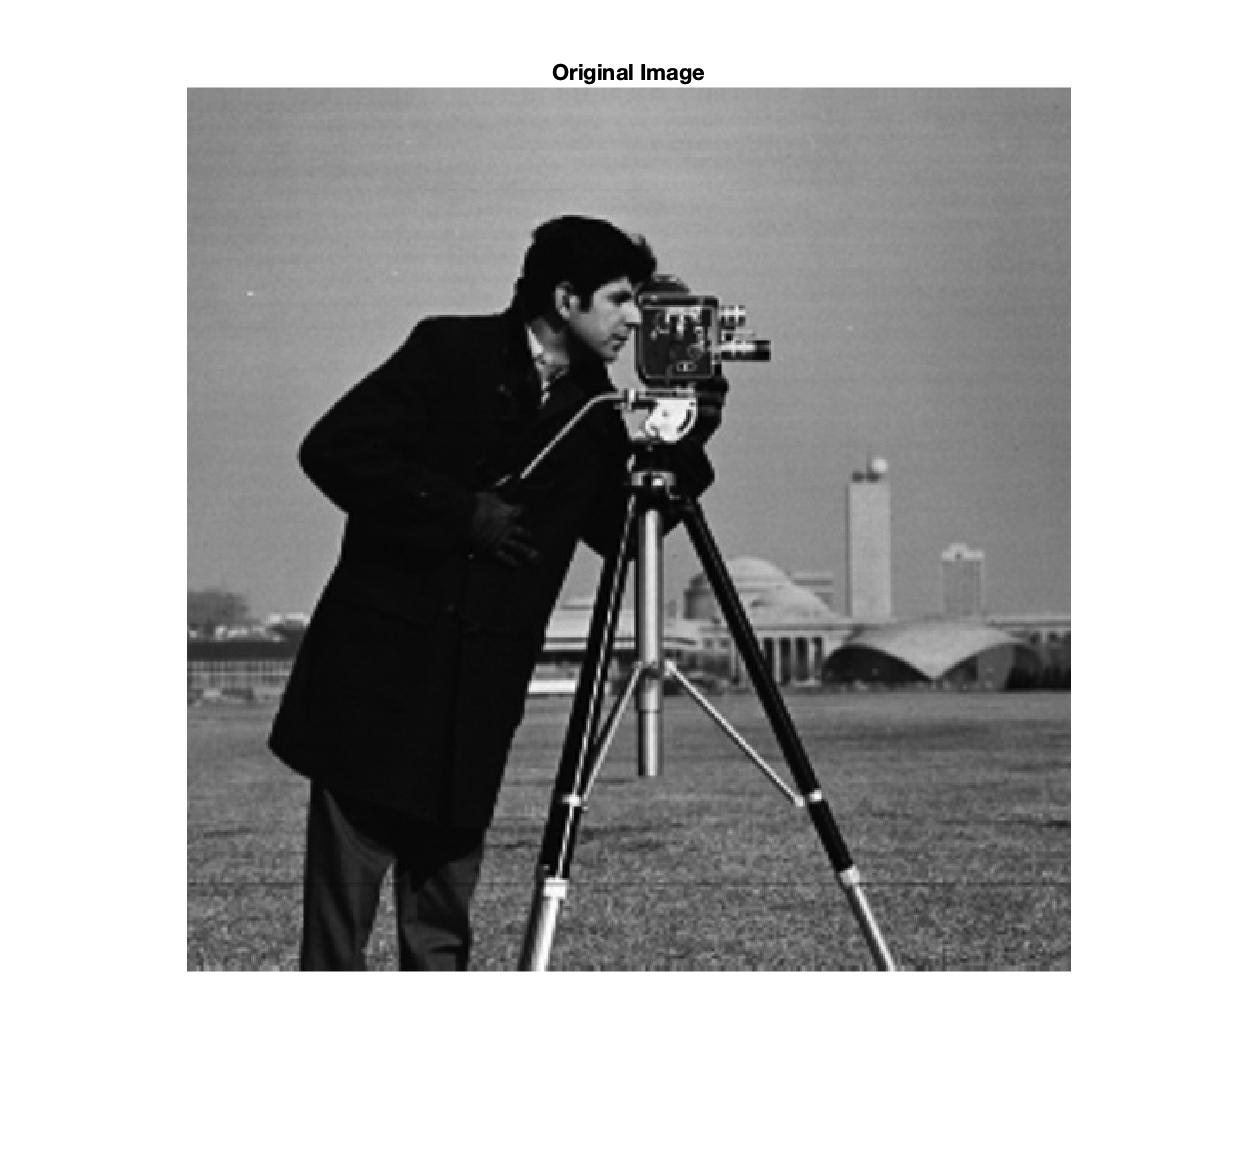
\includegraphics[width=5cm]{cameraman.jpg} }
    }
    \quad
    \subfloat[The first $64$ patches]{
        {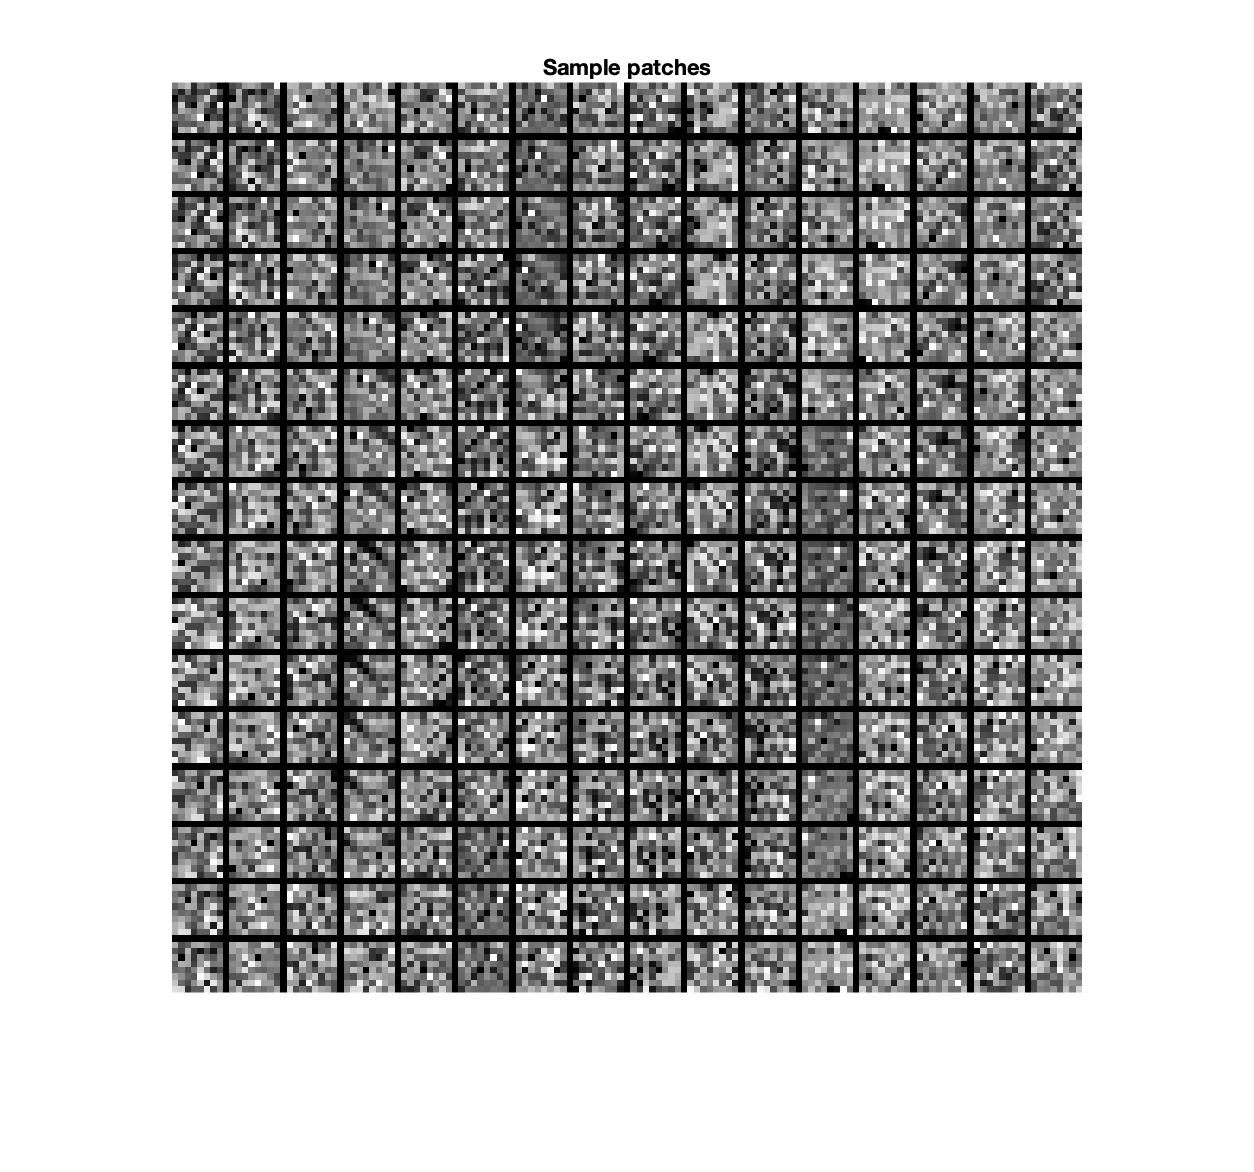
\includegraphics[width=5cm]{cameraman_patches.jpg} }
    }
    \caption{The Camera Man image and its patches}
    \label{fig:cameraman}
\end{figure}
  
In denoising and computer vision, it is common to represent an image as a linear combination of vectors in $\mathbb{R}^n$, to be more concrete an image can be represented as a linear combination of the small image patches of $\sqrt{n} \cross \sqrt{n}$, n is typically $64$ and therefore the patch size is typically $8 \cross 8$ pixels. Figure \ref{fig:cameraman} (a), shows the original picture and Figure \ref{fig:cameraman} (b), shows the first $64$ image patches extracted from the picture. The actual number of patches is proportion to $O(M \cross N)$.

\begin{figure}[h]
    \centering
    
    {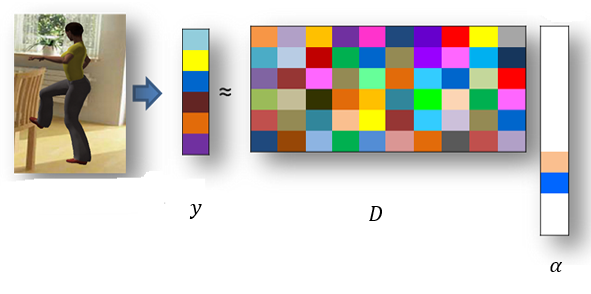
\includegraphics[width=8cm]{sparse_dict_y.png} }
    
    \caption{Sparse coding of an image}
    \label{fig:sparcecode}
\end{figure}

Let's look at the model $\bm{y}=\bm{D}\alpha$ and interpreter it as a way of constructing the image signal $\bm{y}.$ A simple visualization is shown in Figure \ref{fig:sparcecode}. The multiplication of $\bm{D}$ by a sparse vector $\bm{\alpha}$ with $||\bm{\alpha}||_0^0 = k_0 \ll n$ produces a linear combination of $k_0$ atoms which generating the image $\bm{y}.$  
\\

A measured and probably degraded image $\bm{y}$ can be represented as
 \[ 
 \bm{y}=\bm{Hx}+\bm{v}
 \]


Where $\bm{x}$ is the original image we're trying to recover, $\bm{H}$ is a degradation operator, and $\bm{v}$ is an additive linear noise term. If the degradation $\bm{H}$ matrix is set to the identity matrix $\bm{I}$ we have  $\bm{Y} = \bm{x} + \bm{v}$ and the problem reduces to the denoise problem.  To perform denosing is to recover the original signal $\bm{x}$ from the measured signal $\bm{y}$. The idea of the sparse representation is to represent the reconstructed, or the recovered image, $\hat{\bm{x}}$, by the product of a fixed and overcomplete matrix (also known as dictionary) $\bm{D}$ and a sparse and random vector $\bm{\hat{\alpha}}$
\[
    \hat{\bm{x}} = \bm{D}\hat{\bm{\alpha}} 
\]

To find the optimal $\bm{\hat{\alpha}}$ given $\bm{D}$ we need to solve the following optimization problem:
\[
    \hat{\bm{\alpha}} = \argmin_{\bm{\alpha}}||\bm{\alpha}||_0 \quad
    \textrm{s.t.} \quad
    ||\bm{y}-\bm{D}\bm{\alpha}||\le \epsilon
\]
\[
    ||\hat{\bm{\alpha}}||_0 \le||\bm{\alpha}||_0 \implies \hat{\bm{\alpha}} = \bm{\alpha}
\]

where ${\epsilon}$ is a is a predefined error bound that controls the deviation of the observed image $\bm{y}$ from the estimated original image $\hat{\bm{x}}$. 
\\

In previous sections, we discussed the OMP algorithm for solving the sparse vector $\hat{\bm{\alpha}}$ of a known dictionary and commonly used dictionaries includes wavelets, Fourier transformation basis, and Discrete Cosine Transformation (DCT) basis (as shown in Figure \ref{fig:cameraman_dict} (a)). However, such basis may be optimal for certain signals but they may not be the best choice for all kinds of signals, therefore, depending on the application, a data dependent dictionary may be the best choice.  To find a data depend dictionary we need to reformulate our sparse problem to simultaneously solve the sparse vector $\hat{\bm{\alpha}}$ and the dictionary $\bm{D}$:  

\begin{align*}
    \bm{D},\hat{\bm{\alpha}} = \argmin_{\bm{D},\hat{\bm{\alpha}}} ||\bm{y}  - \bm{D}\bm{\alpha}||_F^2 \quad \textrm{s.t.}  \quad ||\hat{\bm{\alpha}}||_0 \le||\bm{\alpha}||_0
\end{align*}

One of the method for solving the problem above is KSVD. The mathematical details of KSVD is beyond the scope of this project, one can refer to the literature in the references section. Basically, the KSVD algorithm attempts to minimize the cost function iteratively, by first finding sparse vector using the OMP algorithm with an initial estimate of the dictionary. This sparse vector minimizes the error in estimation, and at the same time maintain a sparsity constraint as defined in the equation above.  Once this sparse coding stage is done, the algorithm proceeds to update the atoms of the dictionary, one atom at a time, such that the error term is further reduced. Proceeding in such an iterative method, the algorithm reduces the error of estimation at each iteration.
\\

For image processing tasks it is common to use the DCT basis, shown in Figure \ref{fig:cameraman_dict} (a), as the starting dictionary, as the algorithm converges, the DCT basis will look more like patches of edges and textures in the target image as shown in Figure \ref{fig:cameraman_dict} (b). 

\begin{figure}[ht]
    \centering
    \subfloat[The 2D discrete cosine basis]{
        {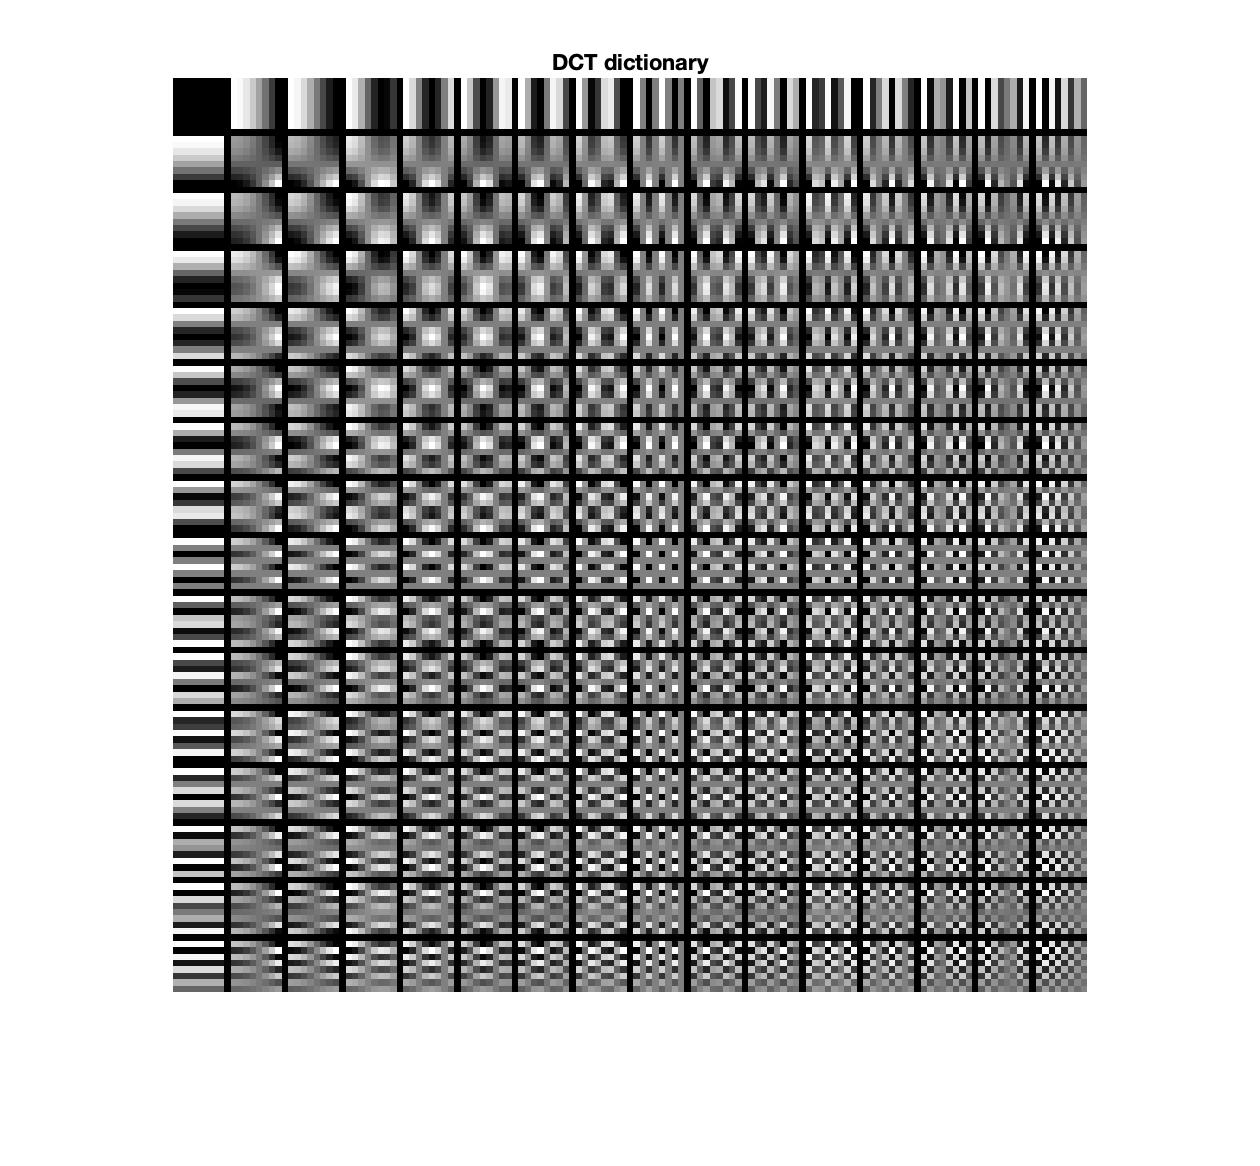
\includegraphics[width=5cm]{cameraman_dct.jpg} }
    }
    \quad
    \subfloat[The learned dictionary from ``The Camera Man'']{
        {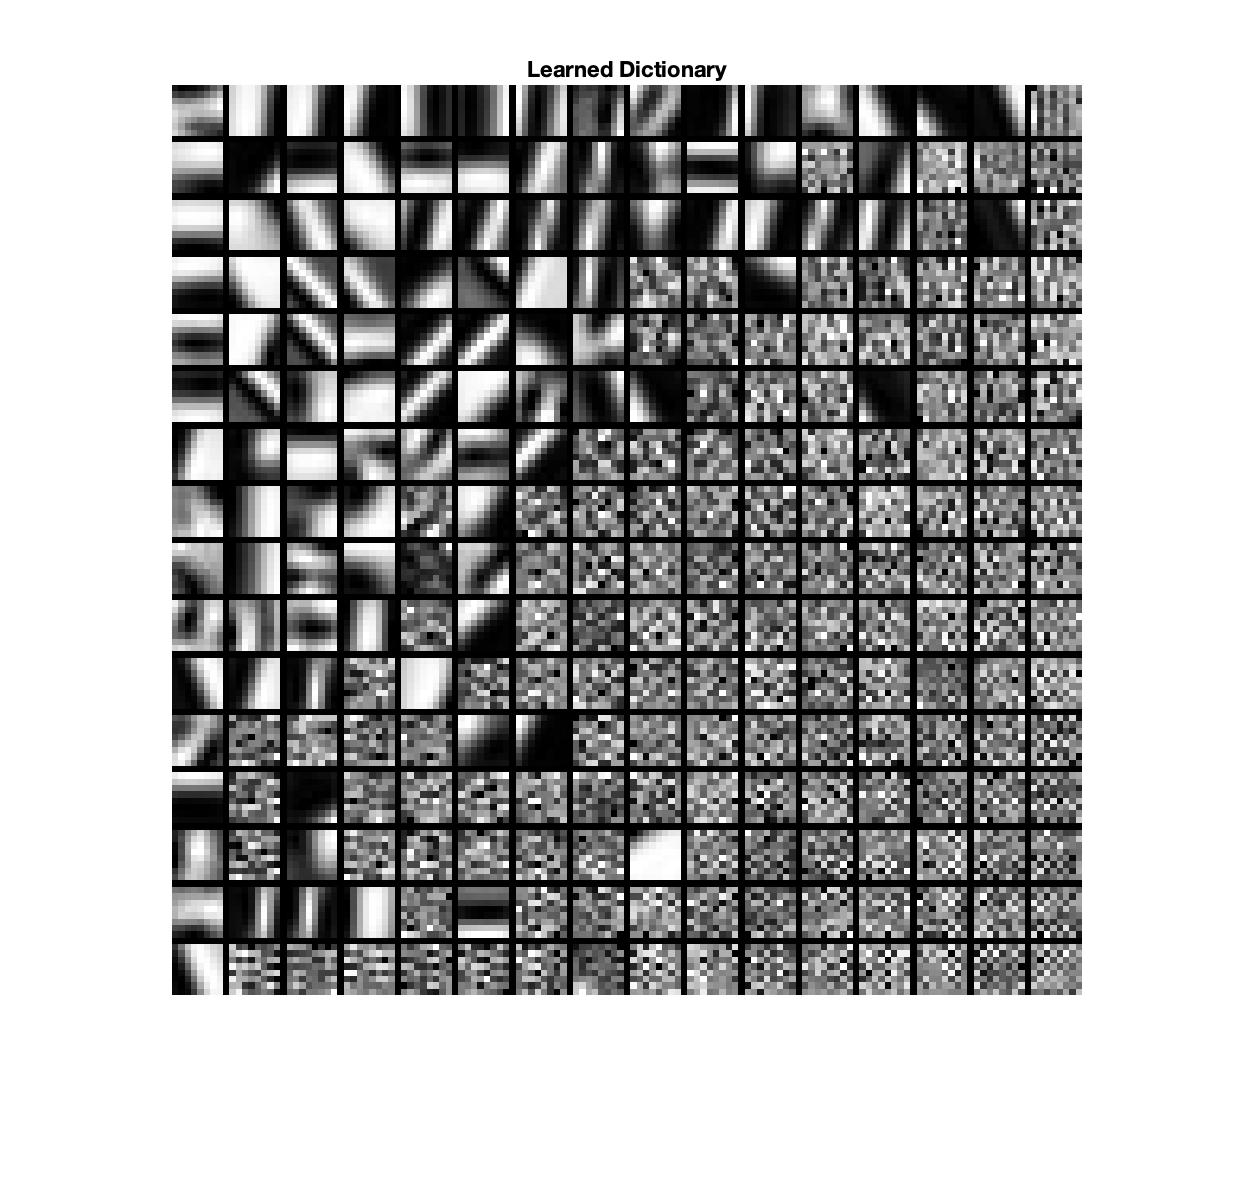
\includegraphics[width=5cm]{cameraman_dict.jpg} }
    }
    \caption{The dictionary}
    \label{fig:cameraman_dict}
\end{figure}  
  
Let's now explorer image denosing with KSVD alogrithm. In your Matlab environment please change the current directory to \texttt{"sparse\_rep/ksvd\_denoise"} directory and open the \texttt{"demo.m"} file. Note, each code section is delineated by a double ampersand  \texttt{"\%\%"} sign. You can click on the section and press the \texttt{"Run Section"} button on the Matlab's toolbar to run only the selected section. 
\begin{enumerate}[1.]
    \item Select and run the \texttt{"Read the image data"} section to view the image. You can change the \texttt{"imgfile"} variable to use a different image in the directory. 
    
    \item Now, let's add some Gaussian noise to the image. Select  and run the \texttt{"Add Gaussian noise with sigma 20"} section. You can experiment different values of $\sigma$ for the Gaussian noise by changing the \texttt{"sigma"} variable. What is the signal to noise ratio (SNR) when \texttt{"sigma=20"} and \texttt{"sigma=35"}?
    
    %Answer: 16.3dB and 11.68dB 
    
    \item Let's run the entire program by clicking the \texttt{"Run"} button on your Matlab's toolbar. 
    \begin{enumerate} [i.]
        \item Inspect the noisy image and the denoised image and comment.
        %Answer: The the denoised image has a higher SNR to the noisy image. However, the denoised image did lose some sharpness compare to the original image. 
        \item Does the error (RMSE) decrease with each iteration? 
        %Answer: Yes the error decreases with each iteration.
        \item What is the SNR on the denoised image? 
        %Answer: 22.35dB
        \item Inspect the initial dictionary (DCT) and the learned dictionary. Give brief comment.
        %Answer: The learned dictionary adopted a lot of features from the image. Specifically, it has learned the some pathes edges, textures and patterns from the image. 
    \end{enumerate}
\end{enumerate}
\pagebreak 

\section*{Appendix}
\subsection*{Solutions to Warm-Up Activity}
\begin{enumerate}[1.]
    \item 

A dictionary is a matrix whose columns are basic vectors, which we call atoms, containing basic information to construct a vector in the same dimension of its column vector.
\item $\bm{\alpha}=\mqty[ 3\\ 2]$
\item $\bm{\alpha}=\mqty[ 2.5\\ 0.5]$ in the first case, and $\bm{\alpha}=\mqty[ 2\\ 1]$ in the second case.
\item The sparsity is 1. Since the column is the first column OMP selected, it is the most similar to our target vector among all columns.
\end{enumerate}
\subsection*{Solutions to Activity}
\begin{enumerate}[1.]
    \item 

We denote by $\bm{A}$ the columns that have been selected by OMP, and residual vector at this step to be $\bm{r}$. Note that the solution vector $\bm{\alpha}$ at this step is updated by solving the least squares problem
\[
||\bm{y}-\bm{A\alpha}||_2^2 \\
\]
Then the solution vector should be
\[
\bm{\alpha} = (\bm{A}^T\bm{A})^{-1}\bm{A}^T\bm{y} \\
\]
And residual vector is
\[
\bm{r} = \bm{y}-\bm{A}(\bm{A}^T\bm{A})^{-1}\bm{A}^T\bm{y} \\
\]
which is the projection of $\bm{y}$ to the space orthogonal to the span of columns of $\bm{A}$.

\item The residual error decreases with more iterations. The decreasing speed is fastest at the beginning, and then slows down with more iterations. This suggest that OMP finds the most related or similar vectors first. The two norm of the residual after $5$ iterations is $4.6$. The sparsity of the solution is $5$, which is controlled by the value of $k$. After $7$ iterations, two norm of the residual is $1.37$, which is less than $10\%$ of the original error $19.62$.
\end{enumerate}

\subsection*{Solutions to Image Denoising}
\begin{enumerate} [1.]
 \setcounter{enumi}{1}
  \item $16.3$dB and $11.68$dB 
  \item
    \begin{enumerate} [i.]
    \item 
       The the denoised image has a higher SNR compare to the noisy image. However, the denoised image did lose some sharpness compare to the original image.
    \item 
       Yes the error decreases with each iteration.
    \item 
       The denoised image has a measurable improvement in SNR. The SNR in the denoised image is $22.35$dB. 
    \item 
       The learned dictionary adopted a lot of features from the image. Specifically, it has learned some patches of edges, textures and patterns from the image. 
    \end{enumerate}
\end{enumerate}
\pagebreak 
\bibliographystyle{plain}
\bibliography{references}
\end{document}